\documentclass{scrartcl}

%\documentclass{report}
\usepackage{braket}
\usepackage{amsmath}
\usepackage{mathtools}
\usepackage{amssymb}
\usepackage{trsym}
\usepackage{pifont}
\usepackage{tcolorbox}
\usepackage[T1]{fontenc}
\usepackage[utf8]{inputenc}
\usepackage[english]{babel}
\usepackage{amsfonts}
\usepackage[super]{nth}
\usepackage{float}
\usepackage{caption}
\usepackage{graphicx}
\usepackage{subcaption}
\usepackage{geometry}
\usepackage{csquotes}
\usepackage{tikz}
\usepackage{circuitikz}
\usepackage{listings}
\usepackage{bbm}
\usepackage{siunitx}
\usepackage{hyperref}
\makeatletter
\renewcommand\paragraph{\@startsection{paragraph}{4}{\z@}%
	{-2.5ex\@plus -1ex \@minus -.25ex}%
	{1.25ex \@plus .25ex}%
	{\normalfont\normalsize\bfseries}}
\makeatother
\setcounter{secnumdepth}{4} % how many sectioning levels to assign numbers to
\setcounter{tocdepth}{4}    % how many sectioning levels to show in ToC
\usetikzlibrary{decorations.pathmorphing}
\geometry{
	a4paper,
	total={150mm,237mm},
	left=30mm,
	top=25mm,
}

\graphicspath{{imgs/}}

\DeclareMathOperator{\var}{Var}

\title{Harmonic Oscillator}
\author{Benedikt Otto}
\subtitle{physics760: Computational Physics}


\begin{document}
	\maketitle

	\newpage

	\tableofcontents

	\newpage

	\begin{abstract}
		To evaluate the behaviour of a quantum particle in a certain potential the path-integral method can be used.
		In this project I investigated the behaviour of particles in a 1 dimensional harmonic and anharmonic potential.
		I measured the ground state energy and the corresponding autocorrelation.
		Additionally I examined the tunnelling behaviour of the anharmonic oscillator for different distances of the minima.
		To verify my code I used the classical limit corresponding to $\hbar \rightarrow 0$.
	\end{abstract}

	\section{Introduction}
		The \textbf{Principle of stationary Action} is a well-known principle in classical mechanics.
		The quantum mechanical generalisation is known as the \textbf{Path integral method}.
		This generalisation does not only take the path with the least action into account, but uses the interference of all possible paths leading to the same final state.
		\\\\
		The harmonic and simple anharmonic oscillators are theoretically well-understood \cite{bender}, the harmonic oscillator is one of the few cases that is analytically solvable \cite{rushka_freericks}.
		The systems used in this work can thus be used to cross-check the validity of the used algorithms.
		Additionally these systems serve as toy models for easy quantum mechanical effects, for example the tunnelling effect.
		\\\\
		The methods used to investigate the harmonic and anharmonic oscillators are the basis for algorithms that are used to examine systems in the QCD.
		More complicated systems, as the quartic interaction $\Phi^4$ and the second quantisation have a similar structure.
		%TODO: add reference

	\section{Theoretical Basis}
		The path integral is given as follows:
		\begin{equation}
			K(a, b) = \int_a^b e^{iS/\hbar} \mathcal Dx(t)
			\label{eq:path_integral}
		\end{equation}
		In equation \ref{eq:path_integral} the integral is performed over all possible paths from point $a$ to $b$, where the quantity $K(a, b)$ corresponds to the probability for this transition.
		The implementation of such a system on a computer leads to problems due to infinite dimensional integrals over infinite boundaries of a quantity with constant modulus.
		Therefore the Euclidean time is used, which is a substitution $t \rightarrow i t$ into imaginary time direction.
		This leads to a rapid decay of paths of little significance.
		\\
		The total action is given by equation \ref{eq:total_action}, in this project the forward derivative is used.
		The constants used in this equation are defined in table \ref{eq:parameters}.
		\begin{equation}
			S = \epsilon \sum_{i=0}^{N - 1} \left(\frac{m(x_{i+1} - x_i)^2}{2\tau^2} + V(x_i)\right)
			\label{eq:total_action}
		\end{equation}
		Because the analysis is more convenient, often periodic boundary conditions are used.
		In this case one can define $x_0 = x_N$, so the right neighbour of $x_{N-1}$ is $x_0$.
		The left part of the equation corresponds to the kinetic energy.
		The velocity used is the average velocity, when the particle moves from site $x_i$ to $x_{i+1}$.
		Because every change only affects three terms, it is not necessary to recalculate the complete action for every change.
		\begin{equation}
			\begin{split}
				\Delta S(x_{i-1}, x_i, x'_i, x_{i+1}) =\\
				\tau\left(V(x_i) - V(x'_i) + m\frac{(x_{i-1} - x_i)^2 + (x_i - x_{i+1})^2 - (x_{i-1} - x'_i)^2 - (x'_i - x_{i+1})^2}{2\tau^2}\right)
			\end{split}
			\label{eq:delta_total_action}
		\end{equation}
		This rewrite reduces the complexity of the problem and improves performance.
		The time complexity per Metropolis iteration is thus reduced from $\mathcal O(N^2)$ to $\mathcal O(N)$, where $N$ corresponds to the number of lattice sites.

		The following parameters will be used and if not otherwise denoted default to the given values:
		\begin{table}[H]
			\centering
			\begin{tabular}{c|l|c}
				parameter & description & default value\\
				\hline
				$i$ & number of Metropolis iterations & 1000\\
				$N$ & number of Lattice sites & 1000\\
				$\tau$ & time distance between steps & 0.1\\
				$m$ & mass of the particle & 0.25\\
				$\hbar$ & value of the reduced Planck constant & 1\\
				$d$ & distance of the minima of the anharmonic potential & -\\
			\end{tabular}
			\caption{Parameters and their default values.}
			\label{eq:parameters}
		\end{table}

	\section{Methods}
	\subsection{Metropolis-Hastings algorithm}
		To generate the track data the \textbf{Metropolis} algorithm is used:

		At first the positions of the particle at every time step is initialised to a random distribution.
		Then for every time step a new position is drawn from a random distribution, in this case from a gaussian distribution.
		If this change lowers the total \textbf{action}, calculated over all the time lattice points, the change is accepted.
		Otherwise, a linearly distributed random value is drawn in the range from 0 to 1 and compared to the exponent of the difference in the \textbf{action}, divided by $\hbar$.
		If the random variable is smaller than the exponential function, the value is accepted, otherwise it is rejected and the position at that time step is not updated.
		This behaviour leads to the tendency to thermalise, but takes care of the quantum behaviour of the particle.

	\subsection{Autocorrelation}
		Since the Metropolis algorithm produces autocorrelated data, this has to be taken into account.
		The estimator of the autocorrelation function is defined as
		\begin{equation}
			\bar C(t) = \frac 1{N} \sum_{i = 1}^{N} (x_i - \bar x_N)(x_{i + |t|} - \bar x_N)
			\label{eq:autocorrelation}
		\end{equation}
		In this case since I always use periodic boundary conditions, that's why one can sum until $N$.
		For $i + |t| > N$ one then has to define $x_{i + |t|} = x_{i + |t| - N}$.
		The normalised autocorrelation function estimator is then defined as:
		\begin{equation}
			\bar\Gamma(t) = \frac {\bar C(t)}{\bar C(0)}
			\label{eq:normalised_autocorrelation}
		\end{equation}
		The variation of the autocorrelation function estimator is given as:
		\begin{equation}
			\var(\bar\Gamma(t)) = \frac 1N \sum_{i=1}^{t + \Lambda}\left[\bar\Gamma(i + t) + \bar\Gamma(i - t) - 2 \bar\Gamma(i)\bar\Gamma(t)\right]^2
			\label{eq:normalised_autocorrelation_error}
		\end{equation}
		$\Lambda$ is in this case a cut-off value, in the following analysis $\Lambda = 5$ is used.
		The error of the lag 0 value $\bar\Gamma(0)$ is defined as 0, because of the normalisation.

		% integrated autocorrelation time
		To determine how many effective samples one can get from the Metropolis samples, one has to calculate the integrated autocorrelation time.
		It is defined as follows:
		\begin{equation}
			\bar \tau_{int} = \frac 12 \sum_{t = -W_{max}}^{t = W_{max}} \frac {\bar C(t)}{\bar C(0)} = \frac 12 + \sum_{t = 1}^{W_{max}} \frac {\bar C(t)}{\bar C(0)}
			\label{eq:integrated_autocorrelation}
		\end{equation}
		There are different methods to determine the cutoff $W$.
		One possibility is to sum until the first element of $\Gamma(t)$ gets compatible with zero within its error.
		I will use the condition $W_{max} > f \cdot \tau_{int}(W_{max})$ to stop the summation, with f defaulting to $5$.
		The second equality sign is valid, since the first term $\frac {\bar C(0)}{\bar C(0)} = 1$ and is only counted once.
		All other terms are counted twice, since the autocorrelation function is symmetrical around 0.

	\subsection{Implementation}
		At first I implemented the complete algorithm in \textbf{Python}, which leads to a fairly poor performance.
		This could mean that one can only get a bad data quality in a given time.
		Thus I optimised the code for performance by simplifying the energy term and precalculating the random variables.
		This reduced the execution time of around 35\%.
		Since this is still a poor performance, I implemented the main Metropolis algorithm loop in \textbf{C++}, the higher level computation is still done in \textbf{Python}.
		For the interfacing the library \verb!ctypes! is used.
		This change improved the total performance, including the still in Python performed generation of the plots, by a factor of around 8.
		This leads to an improvement of data quality due to the higher output rate of around one order of magnitude.
		The complete source code, including all files related to this project are available under the public github repository \cite{github}.
		To verify that the \textbf{C++} code behaves exactly like the Python version, I created some tests, stored in the branch \verb!verify_C!.
		A short manual is given in the \verb!README.md! file, the directory structure is shown in appendix \ref{sec:directory_structure}.
		\\\\
		A very important quantity is the \textbf{accept-ratio}.
		It measures what ratio of changes that were proposed has been accepted.
		To keep the performance high enough, the accept ratio should be as high as possible, but lower than around 65\%.
		This condition is fulfilled for every dataset that is generated.
		\\\\
		The data is stored as \verb!csv! (comma-separated-values) file, a corresponding \verb!cfg! (config) file is generated to store the parameters used and the accept-ratio.

	\section{Results}
	\subsection{Potential}
		As an example the used potentials are shown for different parameters.
		\begin{figure}[H]
			\centering
			\begin{subfigure}[c]{0.49\textwidth}
				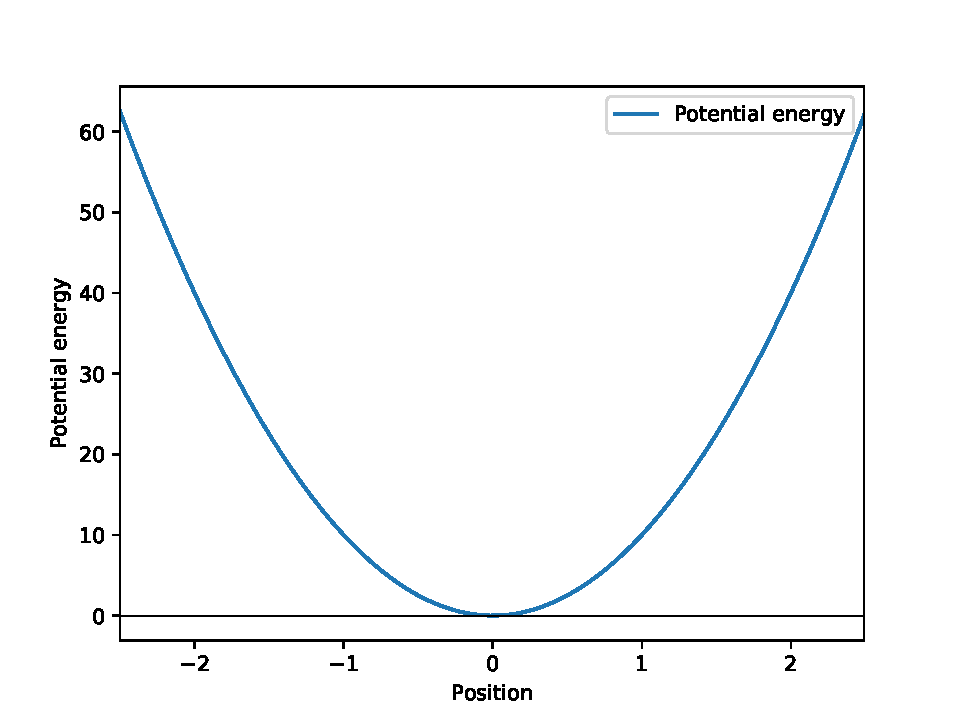
\includegraphics[width=\textwidth]{../imgs/potential/harm_0_0.pdf}
				\caption{Harmonic potential.}
				\label{fig:potential_harm0}
			\end{subfigure}
			\begin{subfigure}[c]{0.49\textwidth}
				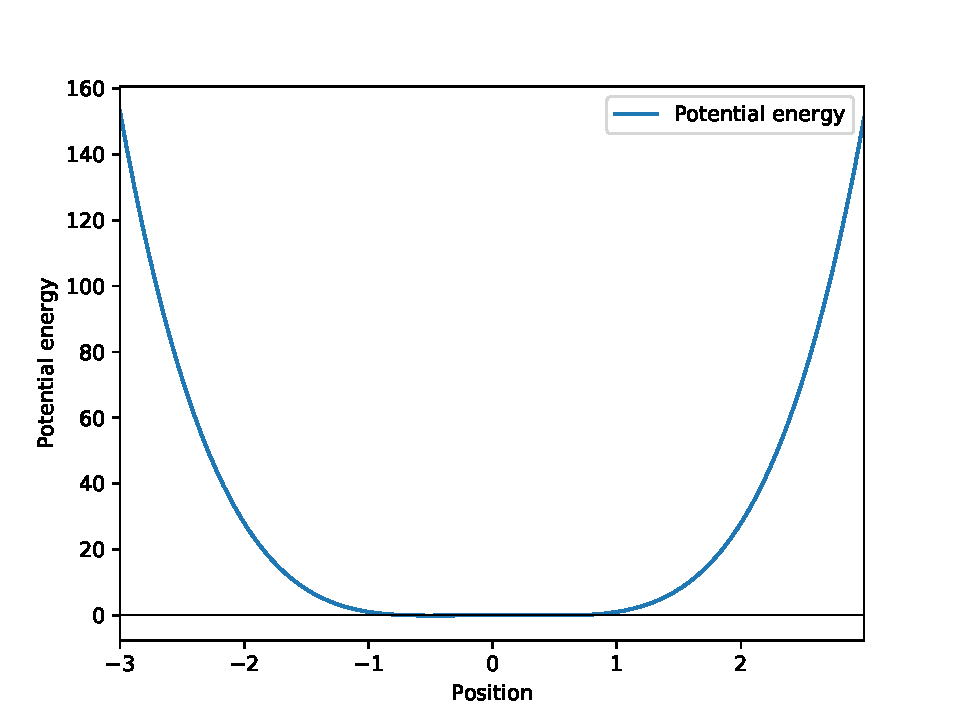
\includegraphics[width=\textwidth]{../imgs/potential/anharm_1_0.pdf}
				\caption{Anharmonic potential, $d=1$.}
				\label{fig:potential_anharm1}
			\end{subfigure}

			\begin{subfigure}[c]{0.49\textwidth}
				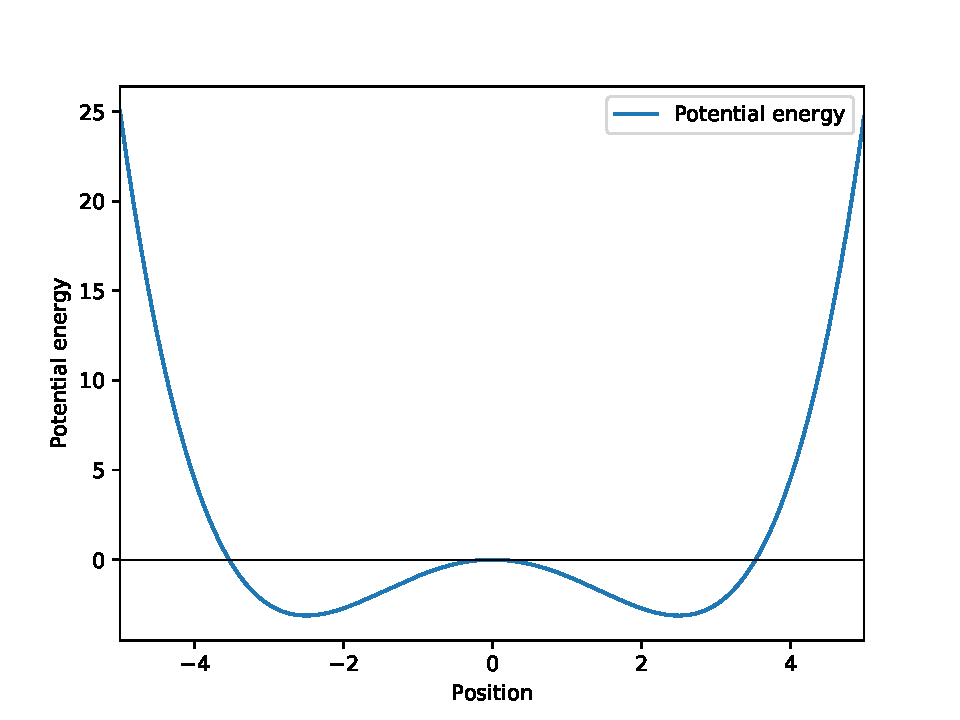
\includegraphics[width=\textwidth]{../imgs/potential/anharm_5_0.pdf}
				\caption{Anharmonic potential, $d=5$.}
				\label{fig:potential_anharm5}
			\end{subfigure}
			\begin{subfigure}[c]{0.49\textwidth}
				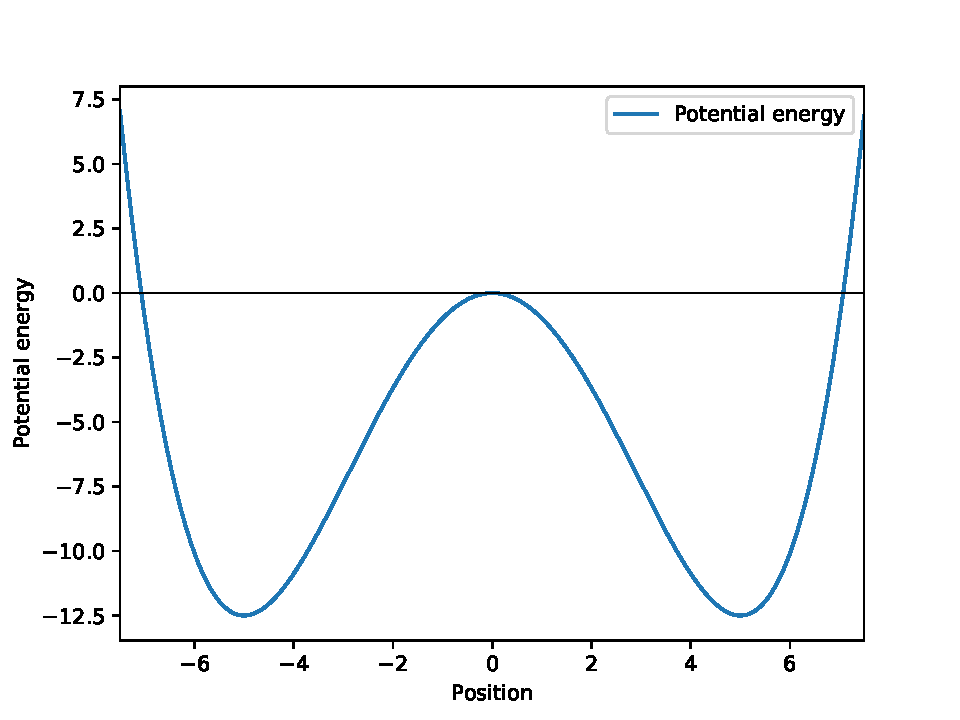
\includegraphics[width=\textwidth]{../imgs/potential/anharm_10_0.pdf}
				\caption{Anharmonic potential, $d=10$.}
				\label{fig:potential_anharm10}
			\end{subfigure}
			\caption{Example potentials.}
			\label{fig:potentials}
		\end{figure}

	\subsection{Verification}
		To verify the validity of the code I performed some tests.

	\subsubsection{Classical limit}
		One of these consistency checks is the classical limit.
		\begin{figure}[H]
			\centering
				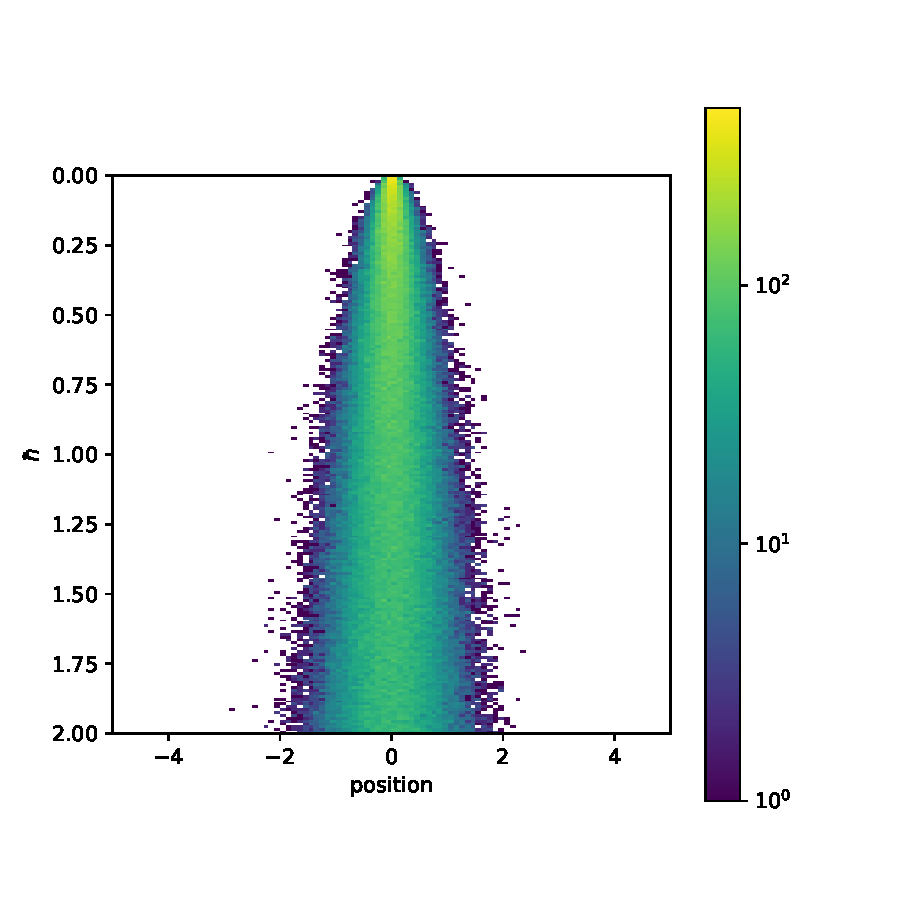
\includegraphics[width=0.6\textwidth]{../imgs/harmonic_oscillator_classical_limit/harmonic_oscillator_10_classical_limit.pdf}
			\caption{Classical limit of the harmonic oscillator.}
			\label{fig:harmonic_oscillator_classical_limit}
		\end{figure}
		In figure \ref{fig:harmonic_oscillator_classical_limit} the standard parameters have been used, on a harmonic potential  with $\mu = 10$ and $\lambda = 0$.
		The parameter $\hbar$ has been varied in the range 0 to 2.

		The same data has been generated for the anharmonic oscillator.
		\begin{figure}[H]
			\centering
				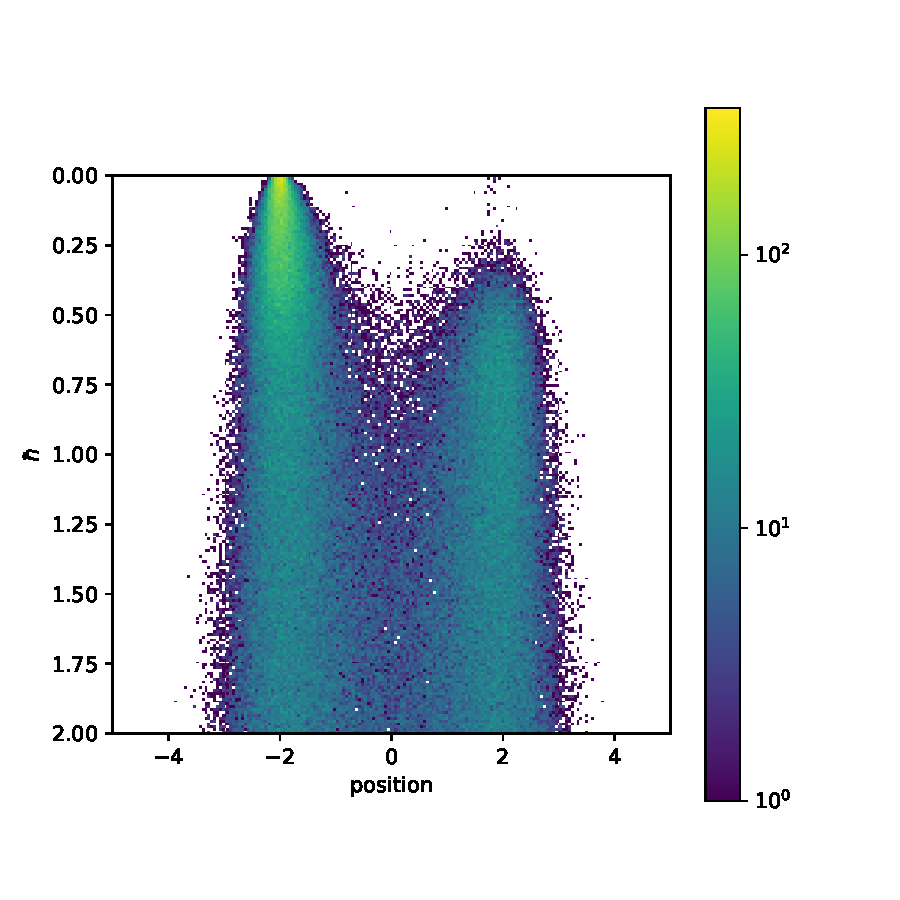
\includegraphics[width=0.6\textwidth]{../imgs/anharmonic_oscillator_classical_limit/anharmonic_oscillator_classical_limit.pdf}
			\caption{Classical limit of the anharmonic oscillator.}
			\label{fig:anharmonic_oscillator_classical_limit}
		\end{figure}
		In figure \ref{fig:anharmonic_oscillator_classical_limit} the following parameters have been used: $i = 200$, $N = 1000$, $m = 0.01$, $\mu = -10.0$, $\lambda = -0.125$, corresponding to a position of the minima at $\pm 2.0$.
		The parameter range for the Planck constant is the same as for the harmonic oscillator.
		The initial state has been prepared into the left minimum.

	\subsubsection{Probability density}
		Another test I performed is to check the shape of the probability density of the harmonic oscillator.
		\begin{figure}[H]
			\centering
				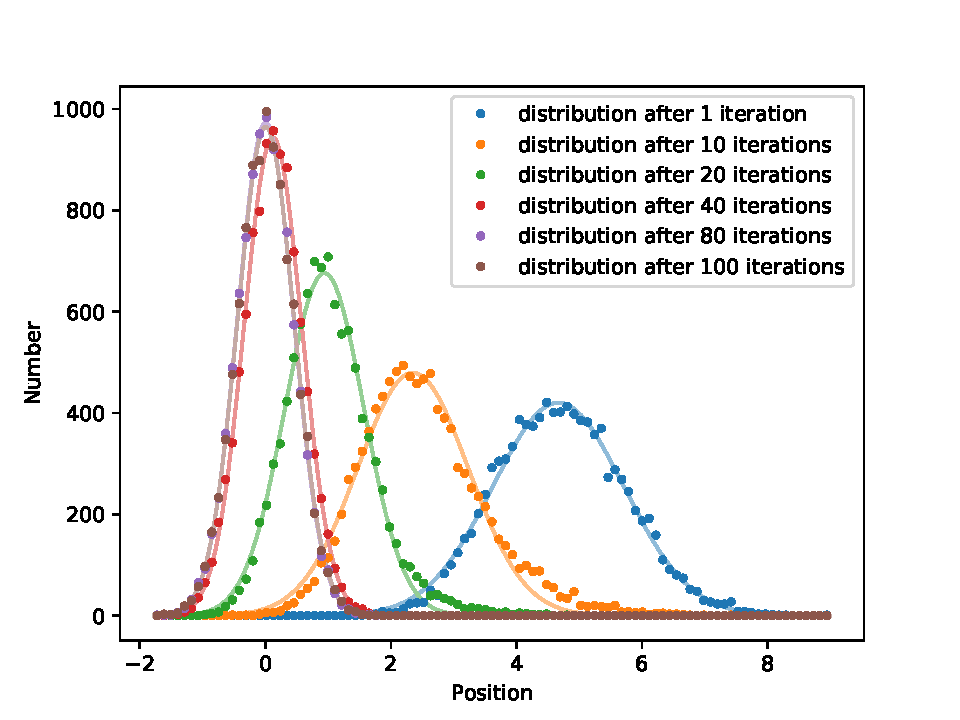
\includegraphics[width=0.6\textwidth]{../imgs/harmonic_oscillator_track/track_10010000_gauss_1_fit.pdf}
			\caption{Probability density for different Metropolis iterations of the harmonic oscillator.}
			\label{fig:harmonic_oscillator_track_10010000_gauss_1_fit}
		\end{figure}
		The parameters used for the plot in figure \ref{fig:harmonic_oscillator_track_10010000_gauss_1_fit} were $i=100$, $N=10000$, $\mu = 10.0$.
		The fits are gaussian distribution functions.
		\\\\
		To investigate further the probability distribution, quantile-quantile plots can be created to compare the distribution with a gaussian shape.
		\begin{figure}[H]
			\centering
			\begin{subfigure}[c]{0.32\textwidth}
				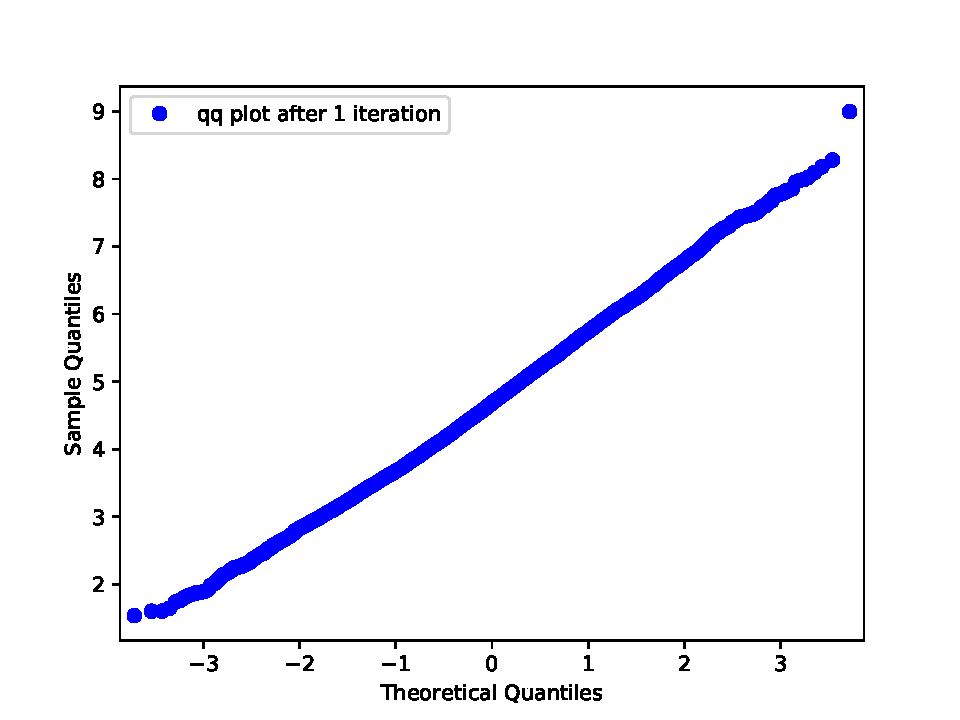
\includegraphics[width=\textwidth]{../imgs/harmonic_oscillator_track/track_10010000_qq_1.pdf}
			\end{subfigure}
			\begin{subfigure}[c]{0.32\textwidth}
				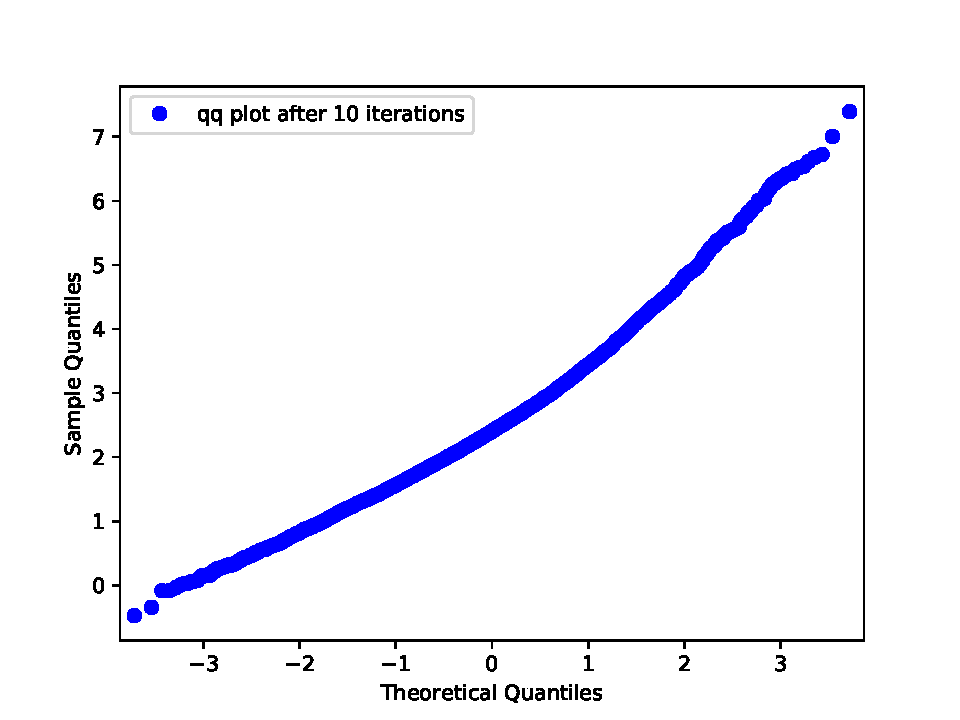
\includegraphics[width=\textwidth]{../imgs/harmonic_oscillator_track/track_10010000_qq_10.pdf}
			\end{subfigure}
			\begin{subfigure}[c]{0.32\textwidth}
				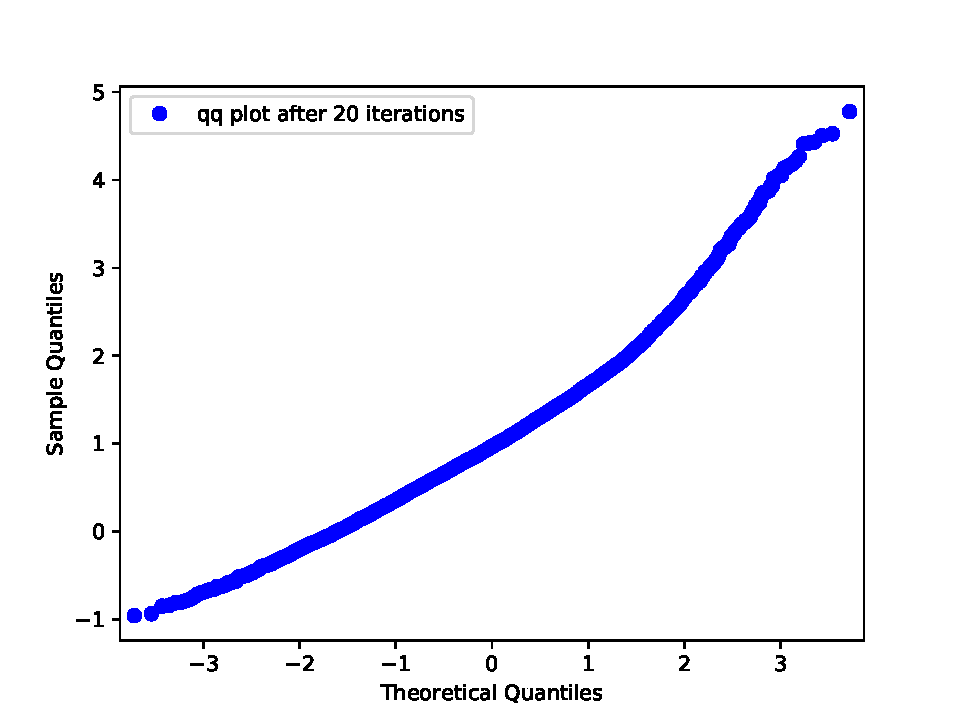
\includegraphics[width=\textwidth]{../imgs/harmonic_oscillator_track/track_10010000_qq_20.pdf}
			\end{subfigure}
			\begin{subfigure}[c]{0.32\textwidth}
				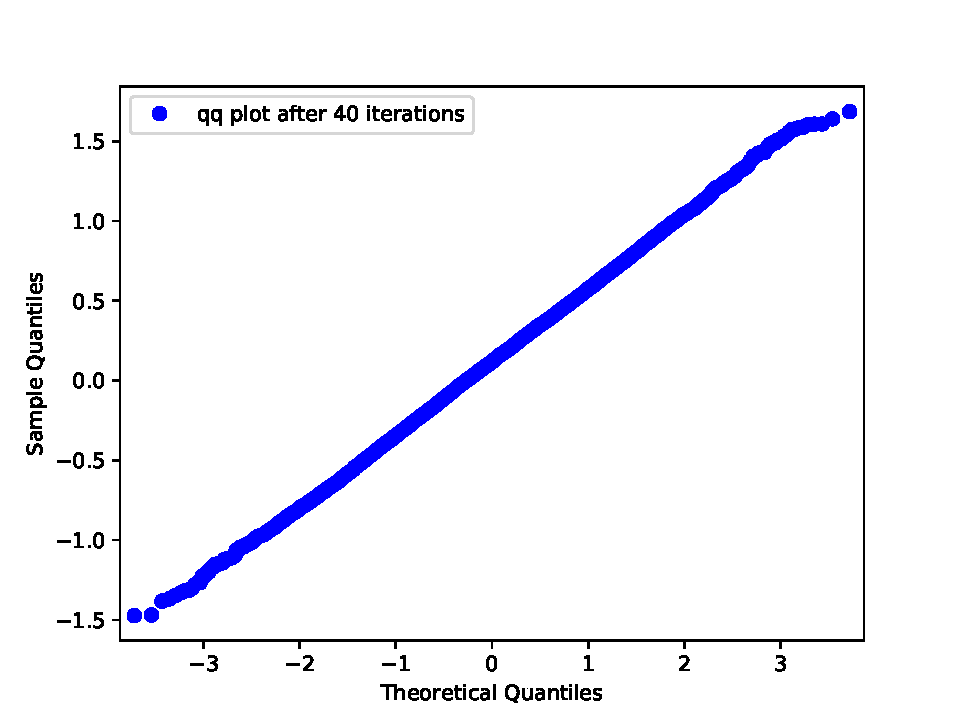
\includegraphics[width=\textwidth]{../imgs/harmonic_oscillator_track/track_10010000_qq_40.pdf}
			\end{subfigure}
			\begin{subfigure}[c]{0.32\textwidth}
				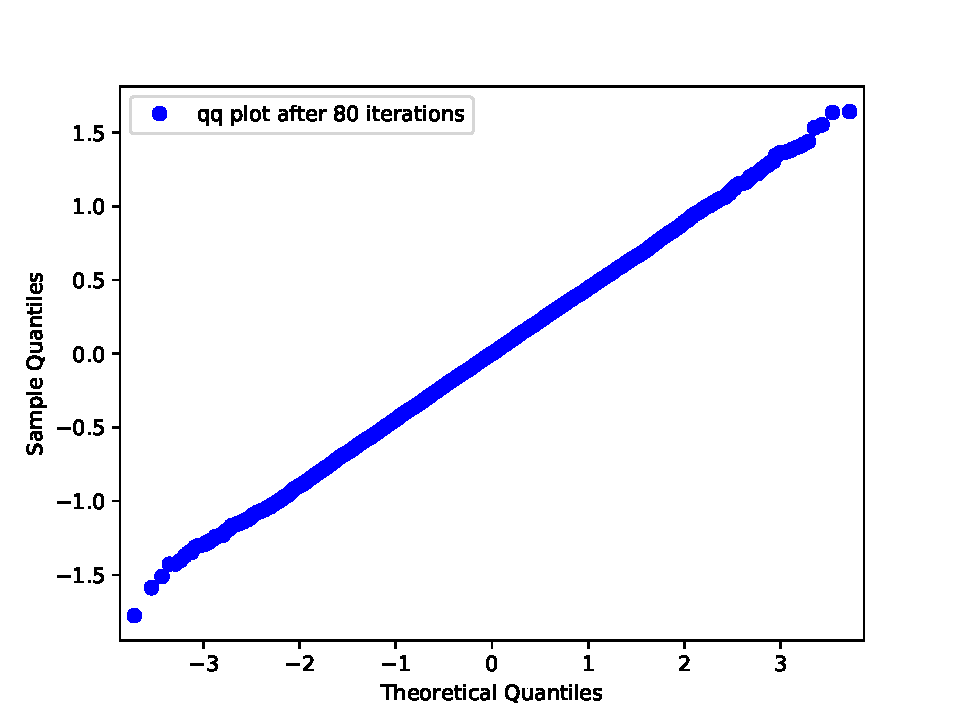
\includegraphics[width=\textwidth]{../imgs/harmonic_oscillator_track/track_10010000_qq_80.pdf}
			\end{subfigure}
			\begin{subfigure}[c]{0.32\textwidth}
				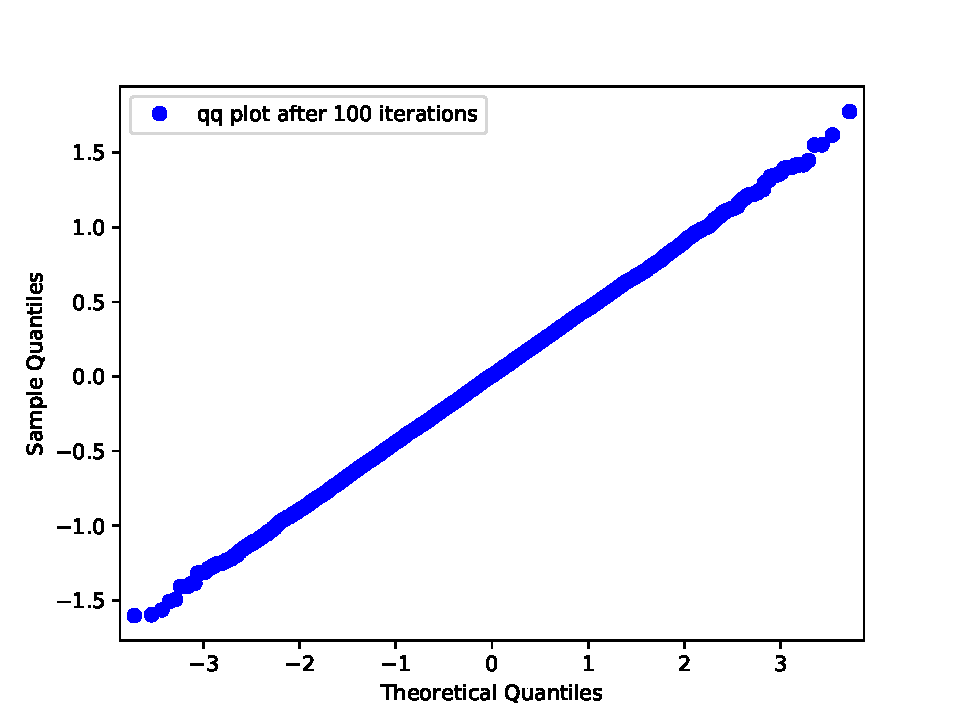
\includegraphics[width=\textwidth]{../imgs/harmonic_oscillator_track/track_10010000_qq_100.pdf}
			\end{subfigure}
			\caption{Thermalisation of the harmonic oscillator from an exited state to the equilibrium.}
			\label{fig:harmonic_oscillator_track_track_10010000_qqs}
		\end{figure}
		In figure \ref{fig:harmonic_oscillator_track_track_10010000_qqs} quantile-quantile plots are shown for the same data and iterations as in figure \ref{fig:harmonic_oscillator_track_10010000_gauss_1_fit}.
		The experimental distribution function was compared to a gaussian distribution function.

	\subsection{Tracks}
		To visualise the behaviour of the particle I created some plots showing the track of the particle.
		\begin{figure}[H]
			\centering
				\begin{subfigure}[c]{0.49\textwidth}
					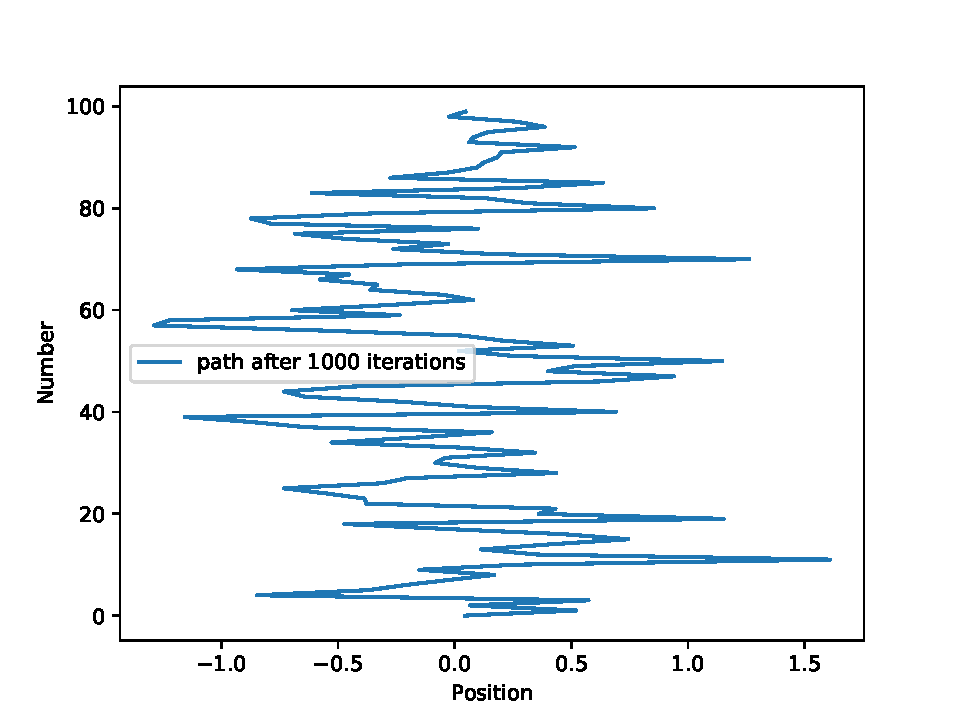
\includegraphics[width=\textwidth]{../imgs/harmonic_oscillator_track/track_1000100_track_1000.pdf}
					\caption{Using a \enquote{light} particle, $m=0.25$}
					\label{fig:harmonic_oscillator_track_1000100_track_1000_light}
				\end{subfigure}
				\begin{subfigure}[c]{0.49\textwidth}
					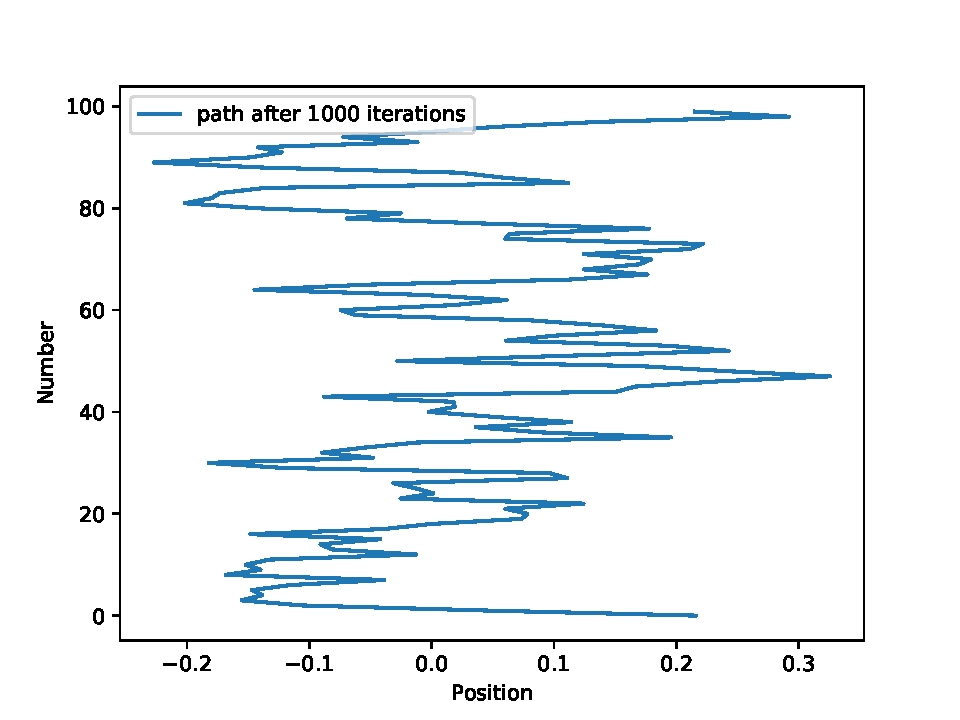
\includegraphics[width=\textwidth]{../imgs/harmonic_oscillator_track/track_1000100_heavy_track_1000.pdf}
					\caption{Using a \enquote{heavy} particle, $m=10.0$}
					\label{fig:harmonic_oscillator_track_1000100_track_1000_heavy}
				\end{subfigure}
			\caption{Typical tracks of the harmonic oscillator.}
			\label{fig:harmonic_oscillator_track_1000100_track_1000}
		\end{figure}
		For the harmonic oscillator one gets a track similar to \ref{fig:harmonic_oscillator_track_1000100_track_1000}.
		The parameters used for the plot were $N=100$, $\mu = 10.0$.
		\begin{figure}[H]
			\centering
				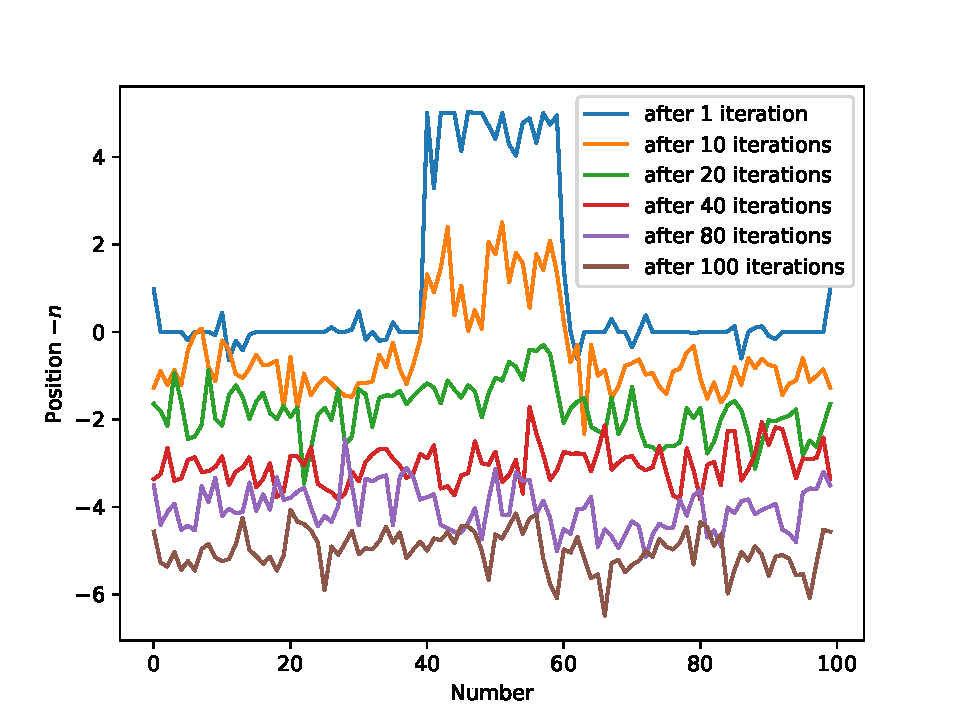
\includegraphics[width=0.6\textwidth]{../imgs/harmonic_oscillator_track/track_100100_step_track_shifted_double.pdf}
			\caption{Typical track of the harmonic oscillator, when initialised with a step function.}
			\label{fig:harmonic_oscillator_track_100100_100100_step_track_shifted_double}
		\end{figure}
		If the initial state is a step function, one gets a plot similar to \ref{fig:harmonic_oscillator_track_100100_100100_step_track_shifted_double}.
		The parameters used for the plot were $i=100$, $N=100$, $\mu = 10.0$.
		The individual tracks are shifted by 1 unit in the y direction, the first iteration is not shifted.
		The track has been prepared with a step function with a width of 20\% in the center and a height of 5.
		The harmonic potential is centred around 0.
		\begin{figure}[H]
			\centering
				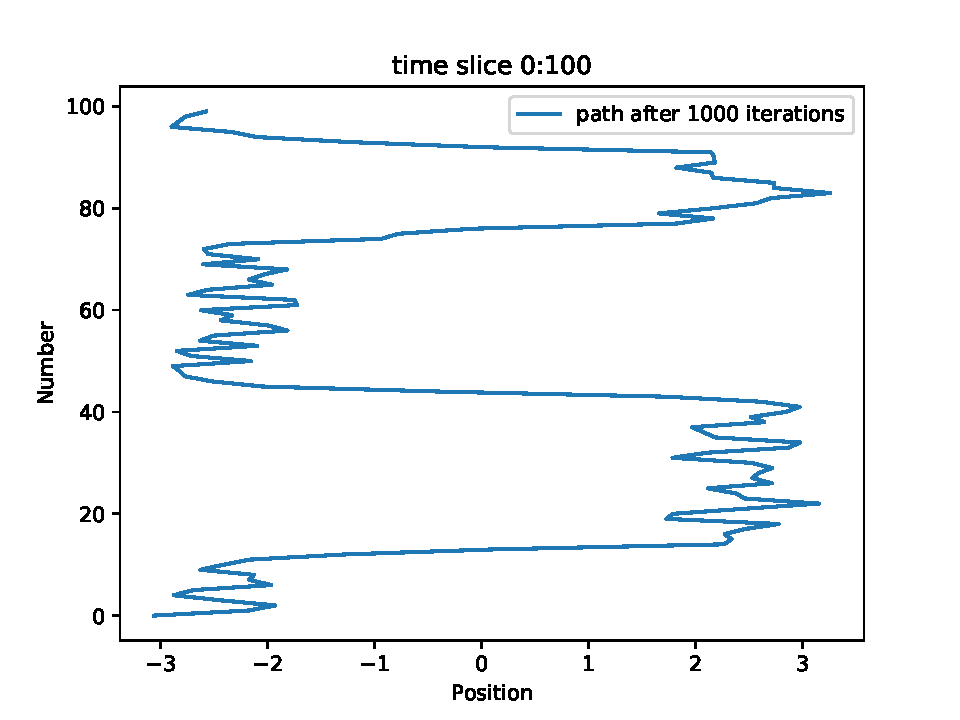
\includegraphics[width=0.6\textwidth]{../imgs/anharmonic_oscillator_track/track_100010005_track_pretty_1000.pdf}
			\caption{Typical track of the anharmonic oscillator, cut to an interesting section.}
			\label{fig:anharmonic_oscillator_track_100010005_track_pretty_1000}
		\end{figure}
		For the anharmonic oscillator one gets a track similar to the one shown in figure \ref{fig:anharmonic_oscillator_track_100010005_track_pretty_1000}.
		The parameters used for the plot were $i=1000$, $N=1000$ but cut to $N=100$, on an anharmonic potential with $\mu = -10.0$, $\lambda = -0.08$, corresponding to a position of the minima at $\pm 2.5$.

	\subsection{Measurements}
	\subsubsection{Classical limit energy}
		\begin{figure}[H]
			\centering
				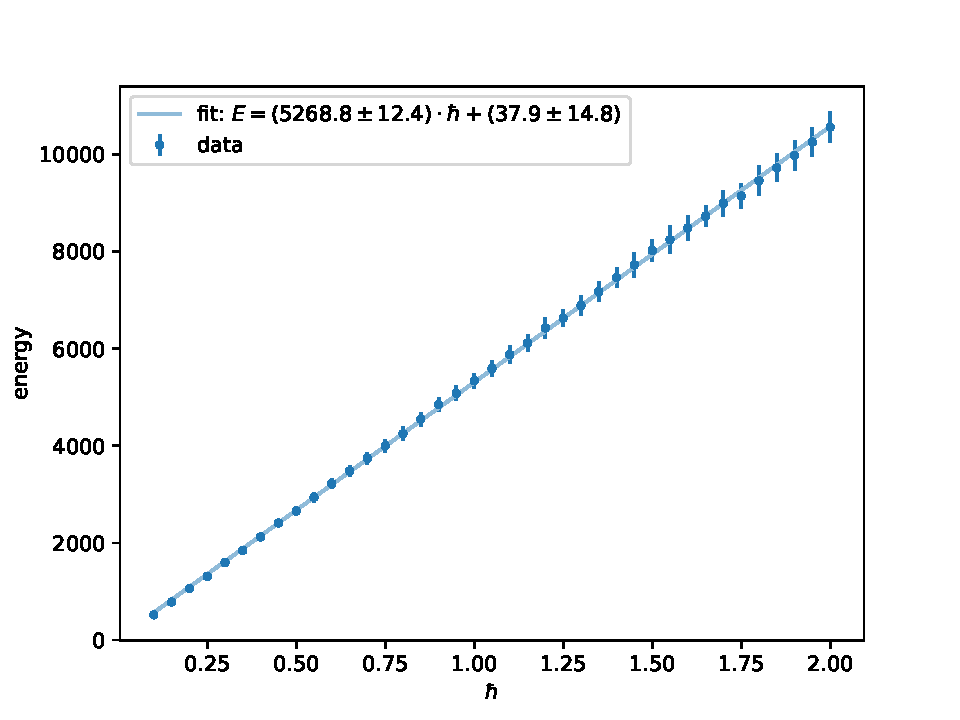
\includegraphics[width=0.6\textwidth]{../imgs/harmonic_oscillator_classical_limit_energy/harmonic_oscillator_10_classical_limit_energy.pdf}
			\caption{Classical limit energy of the harmonic oscillator.}
			\label{fig:harmonic_oscillator_classical_limit_energy}
		\end{figure}
		For plot \ref{fig:harmonic_oscillator_classical_limit_energy} the energy of the harmonic oscillator has been measured depending on the value of $\hbar$.
		The position of the thermalisation has been determined by finding the first sign change of the running mean of the slope of the energy.
		Starting from this position the integrated autocorrelation time has been calculated.
		Then the data has been blocked into blocks of at least $2 \cdot \tau_{int}$, using the upper bound of the error interval, rounded to the next higher integer, from which the energy and standard deviation of the energy has been measured.
		\\\\
		An example is shown for $\hbar = 1$ in figure \ref{fig:harmonic_oscillator_energy_measurement}.

		\begin{figure}[H]
			\centering
				\begin{subfigure}[c]{0.49\textwidth}
					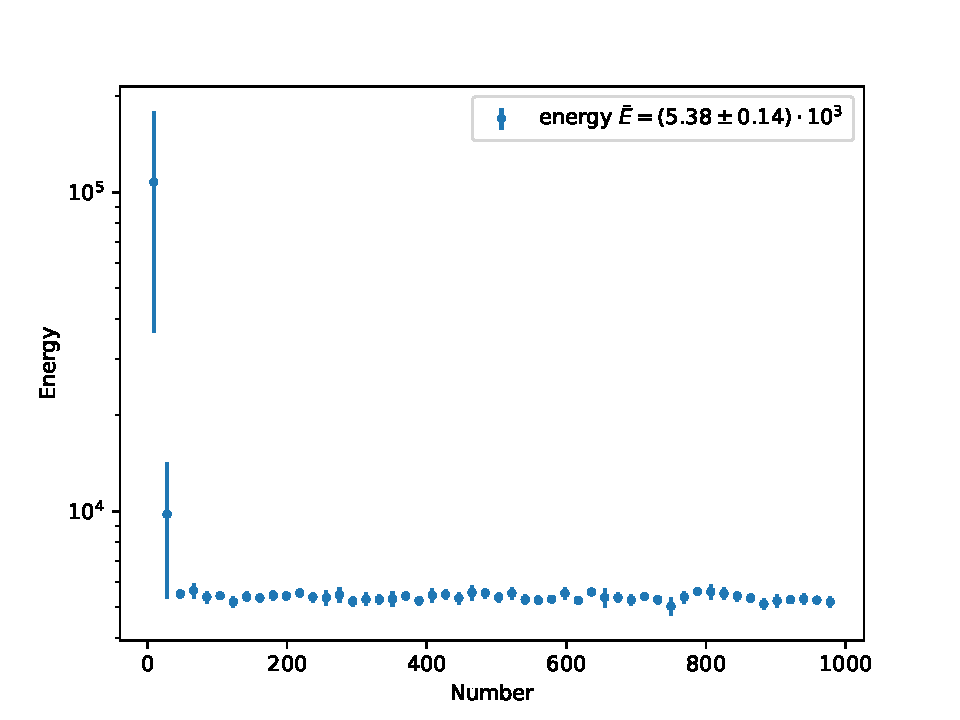
\includegraphics[width=\textwidth]{../imgs/harmonic_oscillator_track/track_10001000_thermalisation_log.pdf}
					\subcaption{Blocked energy measurements}
				\end{subfigure}
				\begin{subfigure}[c]{0.49\textwidth}
					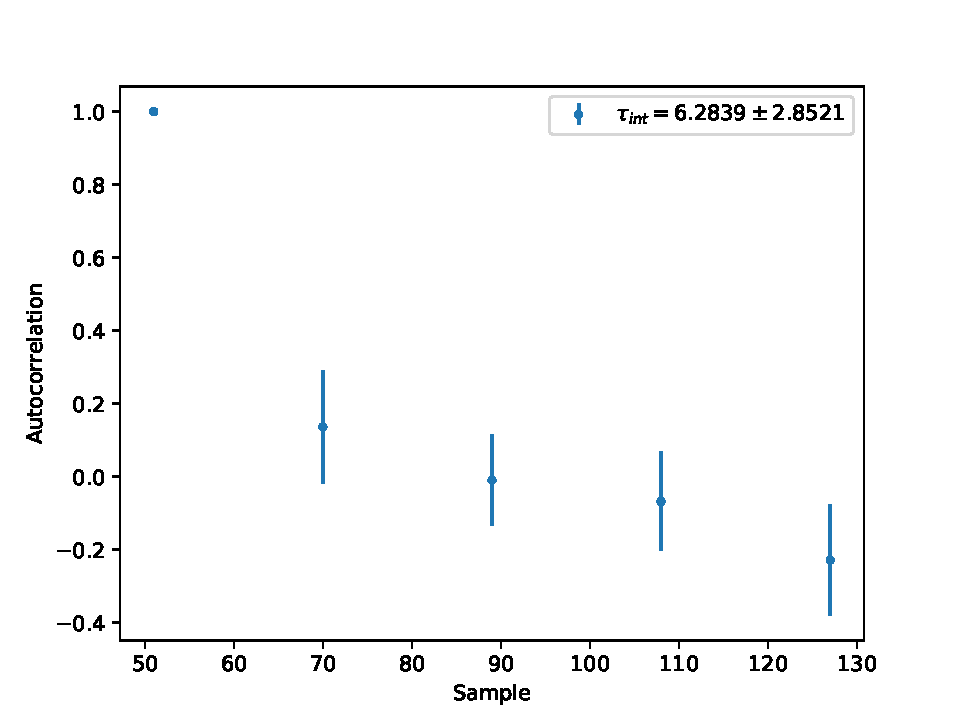
\includegraphics[width=\textwidth]{../imgs/harmonic_oscillator_track/track_10001000_thermalisation_log_autocorrelation.pdf}
					\subcaption{Autocorrelation of the enery measurements}
				\end{subfigure}
			\caption{Measurement of the energy: thermalisation and autocorrelation.}
			\label{fig:harmonic_oscillator_energy_measurement}
		\end{figure}


	\subsubsection{Tunnelling current}
		One of the most interesting features of quantum mechanics is the tunnelling effect.
		\begin{figure}[H]
			\centering
				\begin{subfigure}[c]{0.49\textwidth}
					\includegraphics[width=\textwidth]{../imgs/anharmonic_oscillator_lambda_parameter/track_10001000_tunneling_current.pdf}
					\subcaption{Using 1000 Metropolis iteration.}
					\label{fig:track_10001000_tunneling_current}
				\end{subfigure}
				\begin{subfigure}[c]{0.49\textwidth}
					\includegraphics[width=\textwidth]{../imgs/anharmonic_oscillator_lambda_parameter/track_100001000_tunneling_current.pdf}
					\subcaption{Using 10000 Metropolis iteration.}
					\label{fig:track_100001000_tunneling_current}
				\end{subfigure}
			\caption{Tunnelling current depending on the distance of the classical minima.}
			\label{fig:anharmonic_oscillator_tunneling_current}
		\end{figure}

		\begin{figure}[H]
			\centering
				\begin{subfigure}[c]{0.49\textwidth}
					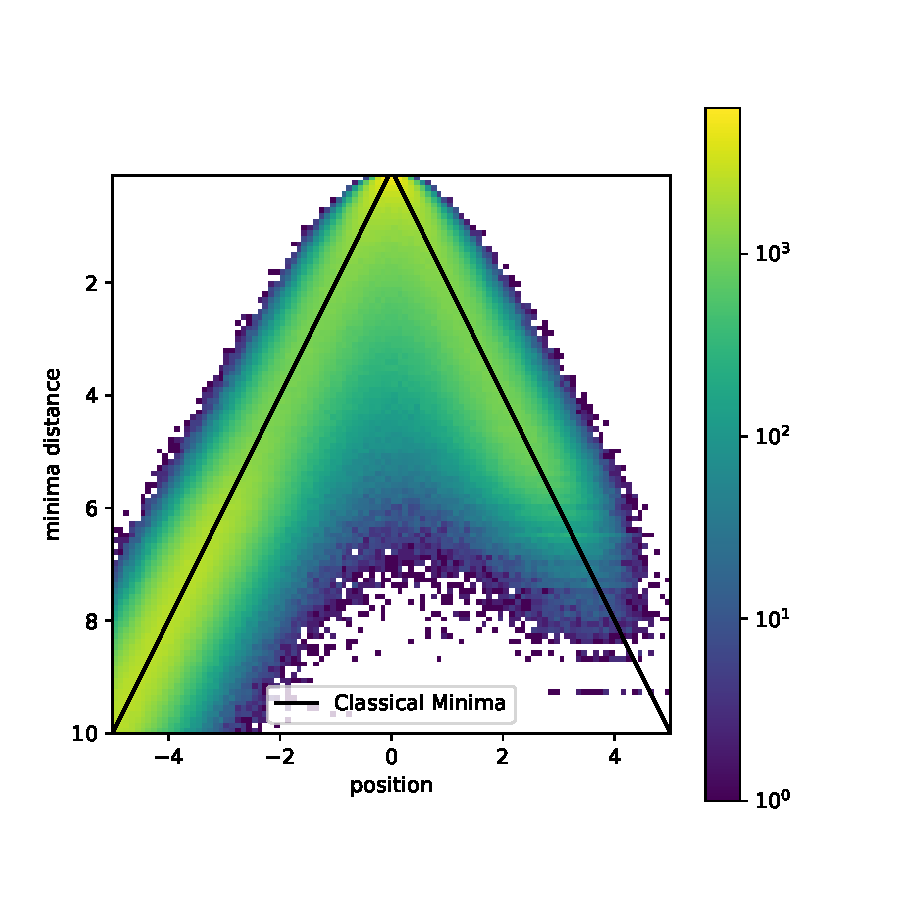
\includegraphics[width=\textwidth]{../imgs/anharmonic_oscillator_lambda_parameter/track_10001000_lambda_parameter.pdf}
					\subcaption{Using 1000 Metropolis iteration.}
					\label{fig:track_10001000_lambda_parameter}
				\end{subfigure}
				\begin{subfigure}[c]{0.49\textwidth}
					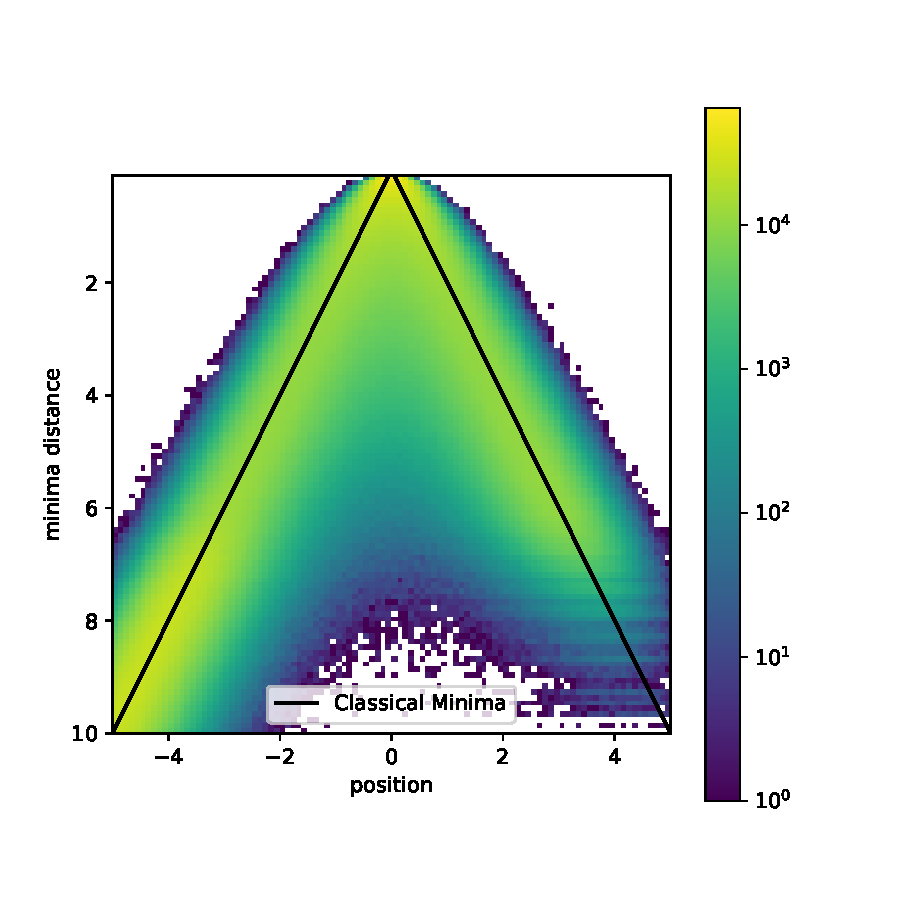
\includegraphics[width=\textwidth]{../imgs/anharmonic_oscillator_lambda_parameter/track_100001000_lambda_parameter.pdf}
					\subcaption{Using 10000 Metropolis iteration.}
					\label{fig:track_100001000_lambda_parameter}
				\end{subfigure}
			\caption{Probability density depending on the distance of the classical minima.}
			\label{fig:anharmonic_oscillator_lambda_parameter}
		\end{figure}
		For plots \ref{fig:track_10001000_tunneling_current} and \ref{fig:track_10001000_lambda_parameter} the following parameters have been used: $\mu = -10$, $\Delta x_{bin} = 0.1$, $\Delta d = 0.1$, with $\Delta x_{bin}$ and $\Delta d = 0.1$ being the size of the bins in position and distance direction respectively.
		For figures \ref{fig:track_100001000_tunneling_current} and \ref{fig:track_100001000_lambda_parameter} the same parameter have been used, except for $i = 10000$ this time.
		In this case every \nth{15} Metropolis iteration has been used, this has been fixed for every value for $\hbar$.
		Otherwise the number of used values per value of $\hbar$ would not be constant.
		For \ref{fig:anharmonic_oscillator_tunneling_current} and \ref{fig:anharmonic_oscillator_lambda_parameter} the same raw data is used.
		The initial state is prepared in the left minimum.

	\subsubsection{Virial theorem}
		It can be shown, that the expectation value of the mean kinetic energy should be equal to the mean potential energy.
		Therefore I checked, if that is the case in this simulation.
		\begin{figure}[H]
			\centering
				\begin{subfigure}[c]{0.49\textwidth}
					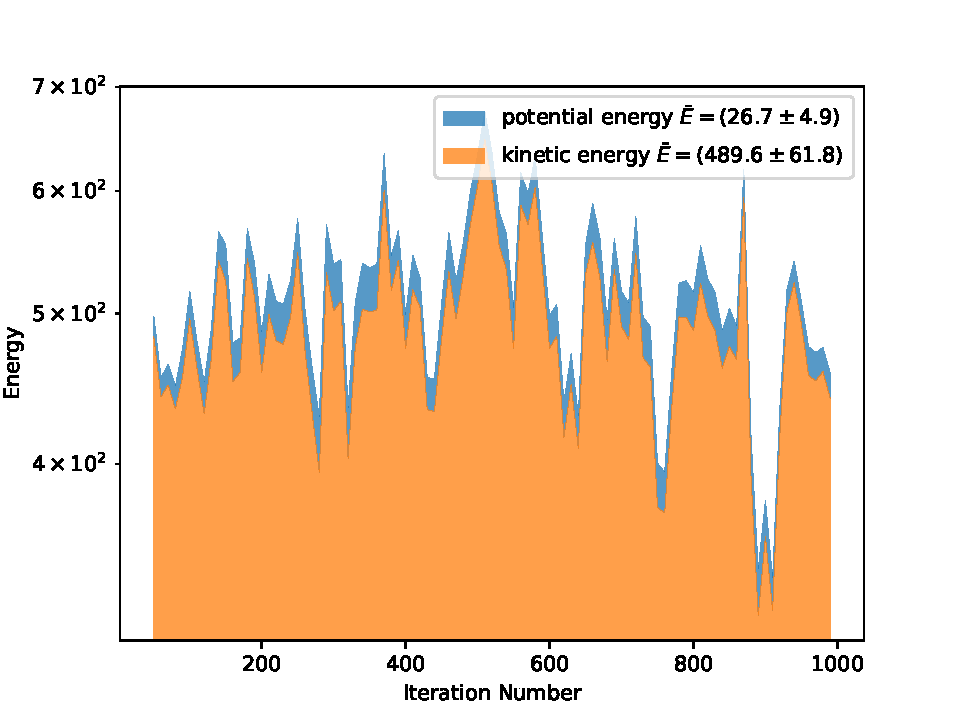
\includegraphics[width=\textwidth]{../imgs/harmonic_oscillator_track/track_1000100_heavy_virial_log.pdf}
					\subcaption{Using $m = 10$.}
					\label{fig:track_1000100_heavy_virial_log}
				\end{subfigure}
				\begin{subfigure}[c]{0.49\textwidth}
					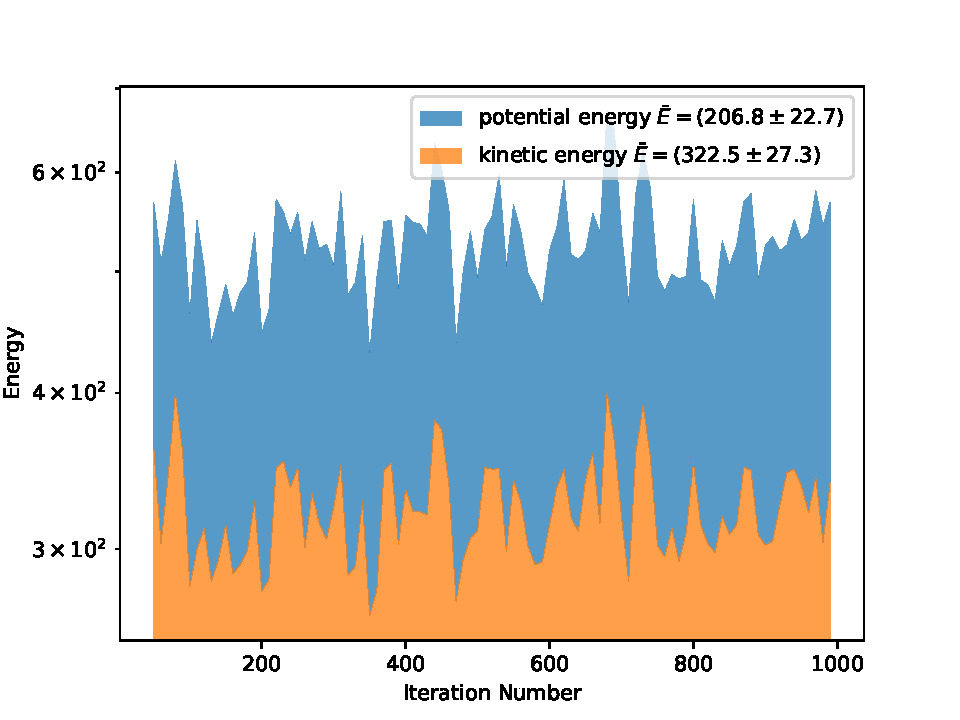
\includegraphics[width=\textwidth]{../imgs/harmonic_oscillator_track/track_1000100_virial_log.pdf}
					\subcaption{Using $m = 0.25$.}
					\label{fig:track_1000100_virial_log}
				\end{subfigure}
			\caption{Distribution of the total energy into potential and kinetic part.}
			\label{fig:track_1000100_virial}
		\end{figure}

	\section{Discussion}
	\subsection{Verification}
	\subsubsection{Classical limit}
		As shown in figure \ref{fig:harmonic_oscillator_classical_limit}, for $\hbar \rightarrow 0$ the probability density collapses into the minimum of the potential, as one would expect from the classical ground state.
		As visible in figure \ref{fig:anharmonic_oscillator_classical_limit}, showing the same plot for the anharmonic oscillator, the behaviour is similar to the harmonic oscillator, such that in the classical limit the probability density only has a significant contribution near the minima of the potential.
		Additionally one observes that there is no significant contribution on the right minimum for $\hbar < 0.3$.
		This is the behaviour one would expect:
		A classical particle in the ground state in potentials used here should state at one of the minima in this case at the left minimum where it was initially prepared.
		Additionally one would expect that the probability for tunnelling tends to zero, which is observable too.

	\subsubsection{Probability density}
		As shown in figure \ref{fig:harmonic_oscillator_track_10010000_gauss_1_fit}, the initial setup was a gaussian shape, centred around the value 5 with a width of 1, visible in the blue curve.
		This corresponds to an exited state, which then thermalises into the ground state.
		The minimum of the potential is centred around 0.
		The distribution then moves towards this minimum, leading to a deviation from the gaussian shape for iterations 10 and 20.
		After 40 iterations the distribution has nearly reached the center of the potential and the distribution becomes again gaussian shaped.
		The difference between iterations 80 and 100 is negligible, this indicates that the thermalisation of the center of mass is done after 80 metropolis iterations.
		From theory one would expect the probability density to be gaussian shaped in the ground state, which is clearly observable as shown below.
		\\\\
		As previously mentioned, one can confirm that the initial setup is a gaussian distribution with center 5 and width 1.
		In the qq-plots for iterations 10 and 20 the deviation from a straight line is clearly visible.
		After the \nth{40} iteration, the center of the distribution has reached 0 and the qq plot matches a straight line, corresponding to a gaussian distribution.
		\\\\
		From these verifications I am confident, that my code is correct.

	\subsection{Tracks}
		In figure \ref{fig:harmonic_oscillator_track_1000100_track_1000} two typical tracks are shown for different particles.
		In figure \ref{fig:harmonic_oscillator_track_1000100_track_1000_light} a very light particle is used.
		This particle performs huge jumps within the potential.
		In contrast to this, the particle used in \ref{fig:harmonic_oscillator_track_1000100_track_1000_heavy} shows a much more continuous track.
		In figure \ref{fig:harmonic_oscillator_track_100100_100100_step_track_shifted_double} one can see how the step function vanishes with increasing Metropolis iteration number.
		The step function disappeared after around 40 Metropolis iterations.
		In figure \ref{fig:anharmonic_oscillator_track_100010005_track_pretty_1000} one sees a part of the anharmonic oscillator track.
		One can clearly see the instants of time when a tunnelling event occurs.

	\subsection{Measurements}
	\subsubsection{Classical limit energy}
		As visible in figure \ref{fig:harmonic_oscillator_classical_limit_energy}, the energy is linearly depending on the value of $\hbar$.
		The fit very well matches the data within error limits.
		This is exactly what one would expect from exact calculation as in $E = \hbar \omega \left(\frac 12 + n\right)$, where $n$ is the state number, in this case $n = 0$ for the ground state.
		$\omega$ is the proportionality factor, depending on the exact shape of the potential.
		In the classical limit $\hbar \rightarrow 0$ one thus gets the correct behaviour $E \rightarrow 0$.
		The slope of the fitted linear function is $\frac\omega2=\SI{5268.8 +- 12.4}{}$.

	\subsubsection{Tunnelling current}
		Plots \ref{fig:track_10001000_tunneling_current} and \ref{fig:track_100001000_tunneling_current} show the rate of tunnelling events divided by the number of possible tunnelling events. %TODO: change
		As visible in figures \ref{fig:track_10001000_lambda_parameter} and \ref{fig:track_100001000_lambda_parameter} real tunnelling only occurs for distances of the minima greater than around 5.
		For smaller distances, the minima of the potential are not clearly separated and transitions are easily possible. %TODO: reference to plot of potential
		For distances greater than 5 one can see, that the tunnelling current decays exponentially with increasing distance.
		\\
		\\
		In figures \ref{fig:track_10001000_lambda_parameter} and \ref{fig:track_100001000_lambda_parameter} is the probability density shown depending on the distance of the classical minima.
		It is obvious, that the distributions for both minima are centred around the positions of the classical minima.
		Comparing \ref{fig:track_10001000_lambda_parameter} with \ref{fig:track_100001000_lambda_parameter}, one can see, that the particle is overrepresented in the right classical minimum for some of the discrete values of $\hbar$.
		This occurs for high distance above around 8.
		The reason for this behaviour is the rapidly decreasing tunnelling current for larger distances of the classical minima.
		Therefore the particle can \enquote{get stuck} in one of the minima.
		If one would like to investigate the behaviour for large distances further, the number of iterations would have to be increased.
		In addition it is clearly visible, that the particle was prepared initially in the left minimum.

	\subsubsection{Virial theorem}
		One thing that I wanted to check, was the \textbf{Virial theorem}.
		For this I measure the kinetic and potential energy separately.
		However, i could not reproduce the \textbf{Virial theorem}.
		The ratio between the energies was very heavily depending on the parameters mass $m$ and the time step size $\tau$.
		Two examples are shown in figure \ref{fig:track_1000100_virial}.
		The ratio between the two parts should be around 1, but the ratios are dependent on the mass and around $17$ and $1.6$.
		Therefore I think that there is an error in the software.

	\section{Summary and Outlook}


	\newpage
	\begin{thebibliography}{widestlabel}
		\bibitem{github} Public Github repository: Harmonic Oscillator, Benedikt Otto (s6beotto), \\\url{https://github.com/s6beotto/Harmonic-Oscillator}.
		\bibitem{latexrun} Public Github repository: latexrun, Austin Clements (aclements), \\\url{https://github.com/aclements/latexrun}.
		\bibitem{rushka_freericks} M. Rushka J. K. Freericks, \textit{A Completely Algebraic Solution of the Simple Harmonic Oscillator}, arXiv:1912.08355 [quant-ph] (2019).
		\bibitem{creutz_freedman} M. Creutz and B. Freedman, \textit{A statistical approach to quantum mechanics}, Annals of Physics, \textbf{132}, 427-462 (1981).
		\bibitem{rodgers_raes} R. Rodgers and L. Raes, \textit{Monte Carlo simulations of harmonic and anharmonic oscillators in discrete Euclidean time}, DESY Summer Student Programme (2014).
		\bibitem{bender} C. M. Bender and T. T. Wu, \textit{Anharmonic oscillator}, Phys. Rev. (2) \textbf{184} (1969), 1231–1260.
	\end{thebibliography}
	\appendix

	\section{Directory structure}
	\label{sec:directory_structure}
	\subsection{Data generation}
	\begin{figure}[H]
		\centering
		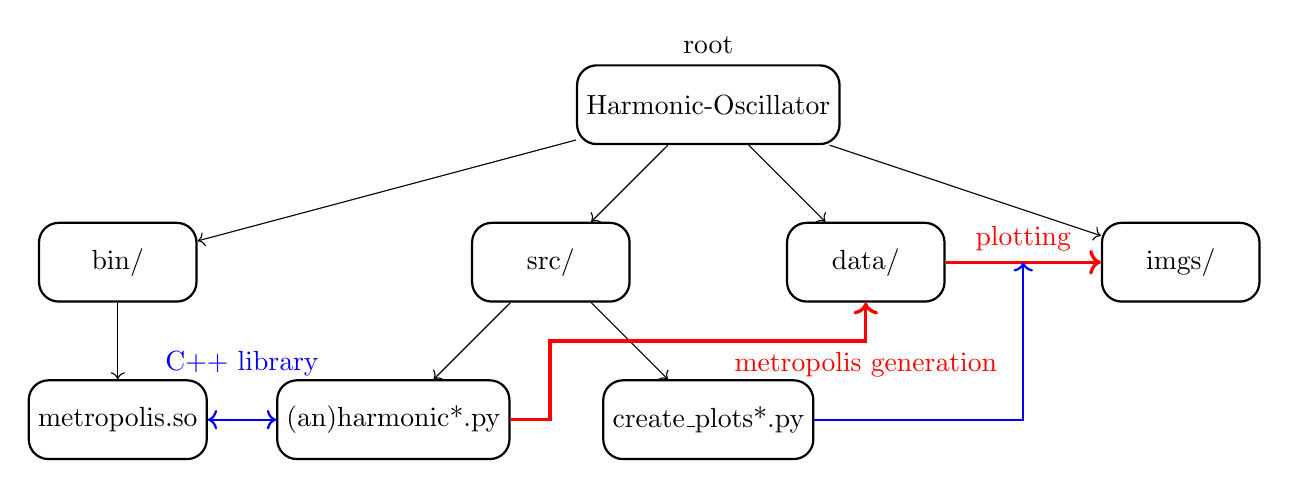
\begin{tikzpicture}
		\draw[color=black, thick]
		node[draw,minimum width=2cm,minimum height=1cm,label=root,rounded corners=0.25cm] (root) at (0, 0){Harmonic-Oscillator}
		node[draw,minimum width=2cm,minimum height=1cm,rounded corners=0.25cm] (bin) at (-7.5, -2){bin/}
		node[draw,minimum width=2cm,minimum height=1cm,rounded corners=0.25cm] (bin_metropolis) at (-7.5, -4){metropolis.so}
		node[draw,minimum width=2cm,minimum height=1cm,rounded corners=0.25cm] (src) at (-2, -2){src/}
		node[draw,minimum width=2cm,minimum height=1cm,rounded corners=0.25cm] (src_create) at (-4, -4){(an)harmonic*.py}
		node[draw,minimum width=2cm,minimum height=1cm,rounded corners=0.25cm] (src_plot) at (0, -4){create\_plots*.py}
		node[draw,minimum width=2cm,minimum height=1cm,rounded corners=0.25cm] (data) at (2, -2){data/}
		node[draw,minimum width=2cm,minimum height=1cm,rounded corners=0.25cm] (imgs) at (6, -2){imgs/};
		\draw [->] (root) -- (bin);
			\draw [->] (bin) -- (bin_metropolis);
		\draw [->] (root) -- (src);
			\draw [->] (src) -- (src_create);
			\draw [->] (src) -- (src_plot);
		\draw [->] (root) -- (data);
		\draw [->] (root) -- (imgs);
		\draw [<->, thick, blue] (bin_metropolis) -- (src_create) node[midway,above=12] {C++ library};
		\draw [->, very thick, red] (src_create.east) -| ++(0.5, 1) -| (data) node[midway,below] {metropolis generation};
		\draw [->, very thick, red] (data) -- (imgs) node[midway,above] {plotting};
		\draw [->, thick, blue] (src_plot.east) -| (4, -2);
		\end{tikzpicture}
		\caption{Directory structure of the project for data generation.}
		\label{fig:scheme_dirs_data_generation}
	\end{figure}

	\subsection{Report generation}
	\begin{figure}[H]
		\centering
		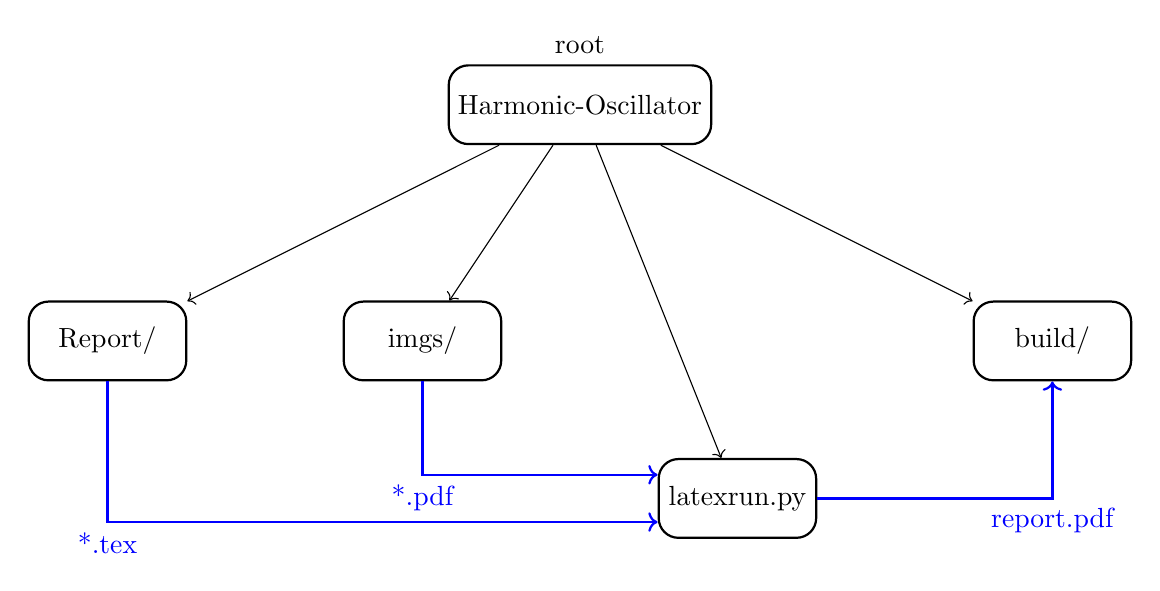
\begin{tikzpicture}
		\draw[color=black, thick]
		node[draw,minimum width=2cm,minimum height=1cm,label=root,rounded corners=0.25cm] (root) at (0, 0){Harmonic-Oscillator}
		node[draw,minimum width=2cm,minimum height=1cm,rounded corners=0.25cm] (report) at   (-6,  -3){Report/}
		node[draw,minimum width=2cm,minimum height=1cm,rounded corners=0.25cm] (imgs) at     (-2, -3){imgs/}
		node[draw,minimum width=2cm,minimum height=1cm,rounded corners=0.25cm] (latexrun) at (2,  -5){latexrun.py}
		node[draw,minimum width=2cm,minimum height=1cm,rounded corners=0.25cm] (build) at    (6,  -3){build/};
		\draw [->] (root) -- (report);
		\draw [->] (root) -- (imgs);
		\draw [->] (root) -- (latexrun);
		\draw [->] (root) -- (build);
		\draw [<-, thick, blue] (latexrun.west) + (0,-3mm) -| (report.south) node[midway,below] {*.tex};
		\draw [<-, thick, blue] (latexrun.west) + (0, 3mm) -| (imgs.south)   node[midway,below] {*.pdf};
		\draw [->, thick, blue] (latexrun) -| (build.south)                  node[midway,below] {report.pdf};
		\end{tikzpicture}
		\caption{Directory structure of the project for report generation.}
		\label{fig:scheme_dirs_report_generation}
	\end{figure}
	The file \verb!latexrun.py! is taken from \cite{latexrun}.
	Every process in the generation of this report is controlled by a makefile.
\end{document}